%%Sorting Networks File. 

%Intro subsection
\section{Sorting Networks}
Let a \emph{wire} be a horizontal line. Let a \emph{comparator} be a vertical line connecting two wires. A 
\emph{sorting network} is a device consisting of $[1 \dots n]$ wires and $[0 \dots m]$  
comparators such that the sorting network sorts a permutation of $n$ elements into ascending order. The 
$n$ elements are first listed to the left of each wire in the network. The elements travel across their respective wires 
at the same time. When a pair of elements, traveling through a pair of wires, 
encounter a comparator, the comparator swaps the elements if and only if the top wire's element 
is greater than the bottom wire's element. A sorting network with $n$ wires and $m$ 
comparators that can sort any permutation of order $n$ is a \emph{complete sorting network}. 
To see a complete sorting network for $n=4$ please refer to Figure~\ref{Fig:SortNetwork}.\par 

\begin{figure}[h]
   ~\centering
    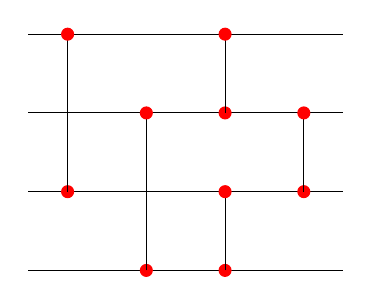
\begin{tikzpicture}
        \draw(0, 0) to (4, 0);
           
        \draw(0, 1) to (4, 1);
        \draw(0, 2) to (4, 2);
           
        \draw(0, 3) to (4, 3);

        %%connector 1
        \draw[red, fill=red](.5,1) circle (.5ex);
            \draw(.5, 1) to (.5, 3);
        \draw[red, fill=red](.5,3) circle (.5ex);


        %%connector 2 
        \draw[red, fill=red](1.5,0) circle (.5ex);
            \draw(1.5, 0) to (1.5, 2);
        \draw[red, fill=red](1.5,2) circle (.5ex);

        %%connector 3
        \draw[red, fill=red](2.5,2) circle (.5ex);
            \draw(2.5, 2) to (2.5, 3);
        \draw[red, fill=red](2.5,3) circle (.5ex);

        \draw[red, fill=red](2.5,0) circle (.5ex);
            \draw(2.5, 0) to (2.5, 1);
        \draw[red, fill=red](2.5,1) circle (.5ex);
        
        %%connector 4
        \draw[red, fill=red](3.5,1) circle (.5ex);
            \draw(3.5, 1) to (3.5, 2);
        \draw[red, fill=red](3.5,2) circle (.5ex);


    \end{tikzpicture}
    \caption{Complete Sorting Network for $n=4$.}
    \label{Fig:SortNetwork}
\end{figure}

Sorting networks were first studied in 1954 by Armstrong, Nelson and O'Connor. 
Sorting networks can be implemented either in hardware or in software~\cite{A18}.
Donald Knuth describes how the comparators for binary integers can be implemented as simple, 
three-state electronic devices~\cite{A18}. Batcher, in 1968, 
suggested using them to construct switching networks for computer hardware, replacing 
both buses and the faster, but more expensive, crossbar switches~\cite{A27}. Since the 2000s, sorting networks are used by the 
\emph{general purpose graphics processing unit community}, which are a group of people who use 
the GPU for non-graphical programming, for constructing sorting algorithms~\cite{A28}.\par 
Sorting networks are intricately related to ladder-lotteries. Let a \emph{minimum sorting network} be defined 
as a sorting network such that for any arbitrary comparator, $c$, on wire $i$, $c$ connects to line $i+1$ or $i-1$. Furthermore, 
the number of comparators in a minimum sorting network is equal to the number of inversions in $\pi$. Clearly there is a 
one to one mapping from the comparators in a minimum sorting network to the bars in an optimal ladder lottery and there 
is a one to one mapping from the wires in a minimum sorting network and the lines in a ladder lottery~\cite{A29}. 


 
\subsection{The Integer Sequence Relating to the Reverse Permutation}
Let $Rev(\pi)$ refer to the reverse permutation of $[1 \dots n]$. There is an integer sequence that counts the number of minimum sorting networks 
for $Rev(\pi$). This integer sequence also counts $OptL\{Rev(\pi)\}$. This sequence grows very quickly, therefore $n=15$ 
is  the largest value this integer sequence has been calculated for. To refer to the table for this sequence 
please refer to Table~\ref{Tab:IntSeq1}~\cite{A30}.
\begin{table}[t]
    \begin{center}

    \begin{tabular}{|p{2cm}||p{8cm}|}
        \hline
        \multicolumn{2}{|c|}{Number of minimum sorting networks/$|OptL\{Rev(\pi)\}|$}\\
        \hline
        n & Count \\ 
        \hline 
        1 & 1 \\
        \hline 
        2 & 1 \\
        \hline 
        3 & 2 \\
        \hline 
        4 & 8 \\
        \hline 
        5 & 62 \\
        \hline 
        6 & 908 \\
        \hline 
        7 & 24698 \\
        \hline 
        8 & 1232944 \\
        \hline 
        9 & 112018190 \\
        \hline 
        10 & 18410581880 \\
        \hline 
        11 & 5449192389984 \\ 
        \hline 
        12 & 2894710651370536 \\
        \hline 
        13 & 2752596959306389652 \\
        \hline 
        14 & 4675651520558571537540 \\
        \hline 
        15 & 14163808995580022218786390 \\
        \hline 
    \end{tabular}
    \end{center}
    \caption{Number of minimum sorting networks and $|OptL\{Rev(\pi)\}|$}
    \label{Tab:IntSeq1}
\end{table}\par
According to Dumitrescu and Mandal, in their paper New Lower Bounds For The Number of Pseudoline Arrangements 
published in 2018, they have devised the current best known lower bound for this sequence to be 
$bn\geq cn^{2} − O(n log n)$ for some constant $c > 0.2083$. In particular, $bn \geq 0.2083 n^{2}$
for large values of $n$~\cite{A33}. Where $bn$ is the bound for a given value $n$. In the paper, Coding 
and Counting Arrangements of Pseudolines by Felsner and Valtr, written in 2011, the authors demonstrate 
the best known upper bound for this sequence is $bn \leq 2^{0.657n^{2}}$~\cite{A32}.\par 

Seeing as there is yet to be a closed form solution for this sequence, new values of $n$ are counted by a variety of algorithms. 
In the paper, Efficient Enumeration of all Ladder Lotteries and its Application, 
the authors were the first to calculate the sequence for $n=11$ with the algorithm {\sc FindAllChildren}~\cite{A1}. 
In the paper, Counting Primitive Sorting Networks by $\mathbb{\pi}$DDs, written by Kawahara, Minato, Saitoh and Yoshinaka, the authors
 were the first to calculate for $n=13$ with a data structure they have termed $\mathbb{\pi}$DD~\cite{A29}. 
 The data structure is a digraph that holds a 
set of elementary permutations along with a number of operations that are applied to the elementary permutations~\cite{A29}.
The data structure resembles a digraph with two sink nodes; one sink node is labelled the zero sink node and the other 
is labelled the one sink node~\cite{A29}.
\pagebreak



